\documentclass[28pt,a4paper]{article}
\usepackage[utf8]{inputenc}
\usepackage{lipsum}
\usepackage{color}
\usepackage{amsmath}
\usepackage{multirow}
\usepackage{multicol}
\usepackage{graphicx}
\usepackage{biblatex}
\usepackage{subfigure}
\usepackage{subcaption}
\usepackage{tikz}
\addbibresource{book.bib}
\title{CSE 300 - Class 1}
\author{Shehabul Islam Sawraz }
\date{\today}

\begin{document}
\maketitle

\section{Introduction}

\begin{figure}[h]
    

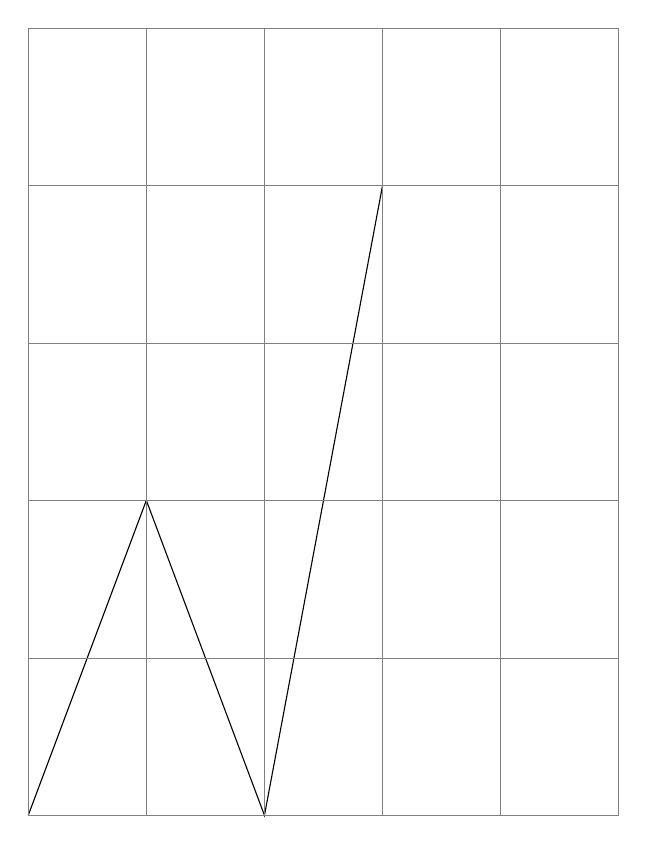
\begin{tikzpicture}[xscale=1.5, yscale=2]

\draw (0,0) -- (1,2) -- (2,0) -- (3,4);

\draw [help lines] (0,0) grid (5,5);

\end{tikzpicture}

\end{figure}

\begin{figure}[h]
    \centering
    \begin{tikzpicture}
    %\draw [|->] (-5,0) -- (5,0);
    %\draw [<->] (0,-5) -- (0,5); 

    %\draw [ultra thick] [<->] (0,5) -- (0,0) -- (5,0);

    %\draw [line width=8] [<->] (0,5) -- (0,0) -- (5,0);

    \draw [red][dotted, thick] [<->] (0,5) -- (0,0) -- (5,0);
    \end{tikzpicture}
    \caption{Caption}
    \label{fig:my_label}
\end{figure}

%Drawing a cure

\begin{tikzpicture}[h]

%\draw [blue] (0,0) rectangle (4,5);
%\draw [ultra thick] (0,0) circle [radius=3];
\draw (7,0) arc [radius=4,start angle=85, end angle=185];

\end{tikzpicture}
\label{fig:my_label}

\begin{tikzpicture}[h]

%\draw [blue] (0,0) rectangle (4,5);
%\draw [ultra thick] (0,0) circle [radius=3];
\draw [very thick] (0,0) to [out=90, in=125] (2,1.5);
\draw [help line] (0,0) grid (2,2);

\end{tikzpicture}
\label{fig:my_label}

\begin{tikzpicture}[h]

%\draw [blue] (0,0) rectangle (4,5);
%\draw [ultra thick] (0,0) circle [radius=3];
\draw [very thick] (0,0) to [out=90, in=180] (2,2) to [out=0, in=90] (4,0) to [out=-90, in=-180] (6,-2) to [out=0, in=-90] (8,0) to [out=90, in=180] (10,2) (10,2) to [out=0, in=90] (12,0) to [out=45, in=225] (14,2);
%\draw [very thick] (2,2) to [out=0, in=90] (4,0);
%\draw [very thick] (4,0) to [out=-90, in=-180] (6,-2);
%\draw [very thick] (6,-2) to [out=0, in=-90] (8,0);
%\draw [very thick] (8,0) to [out=90, in=180] (10,2);
%\draw [very thick] (10,2) to [out=0, in=90] (12,0);
%\draw [very thick] (12,0) to [out=45, in=225] (14,2);
\draw [help line] (0,0) grid (2,2);

\end{tikzpicture}

\begin{tikzpicture}

\draw [domain=0:1.5] plot (\x,{5+\x+\x*\x});

\end{tikzpicture}

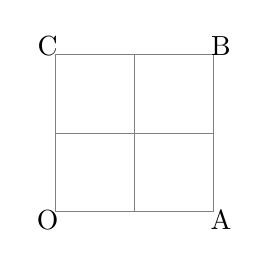
\begin{tikzpicture}

\draw [help lines] (0,0) grid (2,2);
\node at (-0.1,-0.1) {O};
\node at (2.1,-0.1) {A};
\node at (2.1,2.1) {B};
\node at (-0.1,2.1) {C};

\end{tikzpicture}

\begin{tikzpicture}

\draw [help lines] (0,0) grid (2,2);
\node [below left, green] at (0,0) {O};
\node [below right, red] at (2,0) {$A^x$};
\node [above right, yellow] at (2,2) {B};
\node [above left] at (0,2) {$C$};

\end{tikzpicture}



\end{document}